\documentclass{article}

\usepackage[utf8]{inputenc}
\usepackage[T1]{fontenc}
\usepackage{lipsum}
\usepackage{graphicx}
\usepackage{amsmath}
\usepackage[margin=1in]{geometry}
\usepackage{titlesec}

\titleformat{\section}
{\LARGE\bfseries}{\thesection}{1em}{}

\titleformat{\subsection}
{\Large\bfseries}{\thesection}{1em}{}

\begin{document}

\pagestyle{empty}

\section*{Programmazione ad attori}
\large

\textbf{Erlang} è considerato il linguaggio che ha ridefinito la programmazione ad attori, e quando oggi giorno si parla di programmazione ad attori, si pensa semplicemente alla programmazione ad attori così come Erlang l'ha implementata.\\
L'altro linguaggio di programmazione che è interamente all'interno del paradigma di programmazione ad attori è \textbf{Elixir}.\\
Elixir ed Erlang sono praticamente lo stesso linguaggio di programmazione, dove Elixir cambia la sintassi con una sintassi più simile a quelle dei linguaggi più mainstream a cui siamo abituati e aggiunge delle idee, dei costrutti in più rispetto a Erlang. Il cuore del linguaggio e la programmazione ad attori è esattamente quella di Erlang, perché, come vedremo, Erlang ed Elixir condividono lo stesso runtime.\vspace{14pt}\\
La programmazione ad attori è una tecnica per scrivere \textbf{programmi distribuiti}, ovvero programmi che eseguono concorrentemente con thread che possono essere su macchine sparse su una rete. Per fare programmazione distribuita la programmazione ad attori rimane il paradigma più efficace che sia stato mai sviluppato.\vspace{14pt}\\
Sono presenti anche molte librerie per fare programmazione ad attori con molti linguaggi di programmazione mainstream, come ad esemprio librerie per Java e Scala (libreria \textit{H}).\\
Questo approccio però non è sempre consigliato. Quando viene preso un linguaggio di programmazione in cui si cerca di mettere costrutti da due paradigmi, l'idea naïve è che sia una soluzione migliore rispetto ai due paradigmi di partenza, perché è possibile fare una cosa e l'altra, in verità combinare costruti da due paradigmi in generale è problematico.\vspace{14pt}\\
Questo perchè quando viene scritto un frammento di codice, vengono garantite delle proprietà dell'output a partire dalle garanzie presenti sulle proprietà dell'input. Avere a disposizione un linguaggio multiparadigma in cui è possibile unire costruti semplifica la parte di produrre un output e quindi in qualche modo dovrebbe semplificare la parte di produzione di un output con certe garanzie. Il problema è che si va ad indebolire le garanzie in input.\\
Ad esempio, se viene scritto codice in un linguaggio funzionale puro, dove non c'è mutabilità delle strutture dati, si ha la garanzia che il dato non possa essere mutato da qualcun altro. Questo diventa molto importante perché sapere che certe parti del dato non vengono mutate è la chiave che permette di ottenere l'algoritmo con una certa complessità computazionale sintotica nei linguaggi funzionali. Se
si va a mischiare con dei costrutti, ad esempio, imperativi che possono mutare il dato, si va a perdere questa garanzia.\vspace{14pt}\\
Tipicamente un linguaggio di programmazione, un paradigma, viene caratterizzato sia da quello che vi permette di fare, ma anche e spesso soprattutto da quello che \textit{non vi permette di fare}, quindi dalle salvaguardie che vi mette a disposizione.\\
Mischiare paradigmi indebolisce le garanzie e quindi non sempre è la cosa ottimale da fare.\vspace{14pt}\\
Erlang è un linguaggio di programmazione \textbf{funzionale}. All'interno della classe di linguaggi di programmazione funzionale, Erlang si distingue perchè è \textbf{non tipato}, cosa estremamente rara, dato che la maggior parte dei linguaggi di programmazione funzionali oggi giorno sono tipati.\\
Inoltre, Erlang è un po' più di basso livello rispetto agli altri linguaggi simili. In altre parole, bisogna pensare ad Erlang come l'\textbf{assembly} dei linguaggi di programmazione funzionali.\vspace{14pt}\\
Erlang non nasce come linguaggio di programmazione ad attori, ma la riscopre successivamente dopo la sua nascita nel 1976. Oggi, quando si parla di programmazione ad attori, si parla di Erlang.\vspace{14pt}\\
Al centro della programmazione ad attori c'è la nozione stessa di \textbf{attore}. Un attore è caratterizzato da tre ingredienti principali:
\begin{itemize}
    \item \textbf{PID (Process Identifier)}: identificatore univoco dell'attore. E' un \textit{nome logico}. I nomi logici dicono come raggiungere l'attore. Quindi l'unico modo per contattare un attore, se non si sa dov'è perché il linguaggio lo nasconde di natura, è conoscere il nome logico. Quindi solo chi conosce il nome logico di un attore è in grado di comunicare con quell'attore.
    \item \textbf{Mailbox}: coda per la ricezione dei messaggi. L'idea è che un attore riceva dei messaggi e li metta in coda.
    \item \textbf{Behaviour}: mappa che prende i messaggi e li trasforma in una lista di azioni e un nuovo behavior. Ogni volta che viene ricevuto un messaggio, il behavior può cambiare completamente dal precedente. Essendo una mappa, ad ogni messaggio ricevuto corrisponde una lista di azioni ed un nuovo comportamento da rispettare. Per azione si possono intendere anche computazioni interne.
\end{itemize}
L'attore può inviare in maniera asincrona messaggi verso altri attori di cui conosce il PID. L'invio è solamente \textbf{asincrono}, quindi non c'è sincronizzazione. Viene spedito un messaggio e non so se verrà ricevuto o quando verrà ricevuto. Questa è l'unica forma di comunicazione in Erlang. Inoltre, un attore può dare vita ad altri attori.\vspace{14pt}\\
Un attore corrisponde ad un \textbf{unico thread di computazione}, quindi all'interno di un attore non possiamo avere più thread.\\
La programmazione ad attori è un caso particolare di programmazione reattiva o event-driven. Immaginiamo un sistema che abbia decine di migliaia di attori, centinaia di migliaia di attori, milioni di attori. WhatsApp fu implementato inizialmente tramite Erlang. Ogni singola app di WhatsApp installata corrisponde ad un attore. Quindi c'è un attore in esecuzione per ognuno di noi. Erano quindi presenti migliaia di migliaia di attori nel nostro sistema di attori. Gli attori sono normalmente crescenti.\vspace{14pt}\\
Non c'è però l'idea che gli attori stiano facendo calcoli. Quando un attore riceve un messaggio, fa qualcosa per poco tempo, scatenando magari altri messaggi, per poi tornare a fare quelle scelte. Quindi la programmazione ad attori predilige configurazioni in cui ci siano un numero elevatissimo di attori di cui però pochi siano contemporaneamente facenti qualcosa. È il duale della programmazione multithreading dove il numero dei thread deve rimanere basso, piccolo, perché ogni thread sarà costoso e lanciare più thread rallenta significativamente il sistema.\vspace{14pt}\\
Inoltre, gli attori non condividono nulla, non condividono ne stato ne memoria, anche se sono due attori sulla stessa macchina, che magari stanno collaborando fra di loro attraverso scambio di messaggi, non condividono risorse di nessun genere.\vspace{14pt}\\
Un \textbf{sistema di attori} è un sistema complesso composto da più attori in esecuzione. L'esecuzione è indipendente dalla locazione fisica degli attori e la topologia della rete è variabile. Gli attori possono essere eseguiti in maniera totalmente trasparente sullo stesso nodo, sulla stessa Virtual Machine, sulla stesso Core, sulla stessa CPU. Questo vuol dire che in Erlang non c'è di fatto distinzione tra programmazione concorrente su una singola macchina, programmazione distribuita o programmazione parallela.\\
Uno dei punti di forza della programmazione ad attori di Erlang è aver dato una soluzione drastica ma perfettamente funzionante alla gestione dei guasti.

\subsection*{Esempio pratico in Erlang}
Erlang condivide la sua sintassi con il linguaggio di programmazione logica Prolog.\\
Un esempio di attore per la gestione di un conto corrente è il seguente:
\begin{center}
    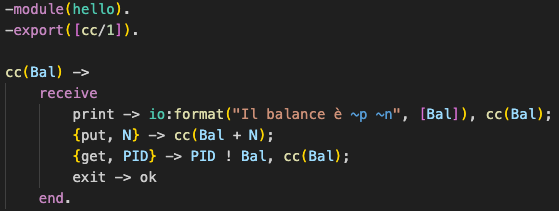
\includegraphics[width=1\textwidth]{img/hello_code.png}
\end{center}
Il primo step è la dichiarazione del \textbf{module}, dove il suo nome deve essere lo stesso del nome del file. In Erlang, quando una riga inizia con il segno \textbf{-} è una divertiva, quindi non fa parte del codice ma aiuta il compilatore a fare qualcosa.\vspace{14pt}\\
Un secondo aspetto è che all'interno di un codice Erlang vengono definite delle funzioni, le quali si può decidere se esportare o meno tramite \textbf{export}. In questo modo è possibile scegliere quali funzioni esportare e quali non esportare. Tutto ciò che non viene esportato è nascosto. La direttiva export prende una lista di funzioni da esportare, dove va dichiarato il nome della funzione / il numero di parametri che richiede in input la determinata funzione. Questo perchè ci possono essere funzioni con lo stesso nome ma differenziate dal numero di parametri.\vspace{14pt}\\
In Erlang, tutte le istruzioni, i comandi, le definizioni, terminano con il \textbf{punto}.\vspace{14pt}\\
Quando definiamo un attore, bisogna definire un behavior. Il behavior deve dire: se ricevo certi messaggi, faccio qualcosa.\\
Il mio conto coerente deve avere un \textit{balance}, che per l'appunto mi dice quanti soldi ho. Una volta ricevuto un messaggio, devo acquisire un nuovo behavior.\\
L'idea di Erlang è che il behavior viene definito da una funzione, una funzione che è tipicamente ricorsiva. Quindi, la mia funzione ricorsiva prenderà in input lo stato, in questo caso prenderà in input il balance attuale, poi descriverà come reagire ai messaggi, e tipicamente, dopo aver ricevuto un messaggio, prenderà un altro behavior.In questo caso, il behavior è sempre quello. Io voglio che il mio conto coerente continui a ricevere messaggi.\vspace{14pt}\\
Erlang non ammette mutazioni di nessun tipo, tranne per un paio di costruttori particolari. Le variabili non possono quindi essere variate, sono praticamente delle costanti.\vspace{14pt}\\
Un behavior viene descritto all'interno di un costrutto \textbf{receive-end}.
Il behavior deve dirmi: se ricevo un certo messaggio, faccio una certa cosa. Vado a scrivere questo tramite una serie di pattern che verranno confrontati con i messaggi nella mailbox in un certo ordine e se nella mailbox viene trovato un messaggio che fa match con un certo pattern, allora viene eseguito un certo codice.\\
Un pattern è una descrizione, una possibile forma dell'input. Quindi, ogni possibile descrizione di un pattern può matchare o no qualcosa che era mailbox, se con la stessa forma. E non solo, nel caso in cui il pattern matchi qualcosa che era mailbox, legherà dei nomi di variabile al contenuto del messaggio.\vspace{14pt}\\
Come sono fatti questi pattern? Il primo e l'ultimo pattern, \textit{print} ed \textit{exit}, corrispondono semplicemente ad avere ricevuto come input print o exit.\\
Anche in questo caso sono scritti con le lettere minuscole, come \textit{cc}, ma non hanno una tonda.
Con la lettera minuscola e parentesi tonde, è una funzione. Senza tonda non è una funzione, ma un \textbf{atomo}.\\
Un atomo è un dato che non ha niente di interessante se non il fatto di essere uguale a se stesso e diverso da tutti gli altri atomi. Lo si può utilizzare per indicare qualcosa, ad esempio l'atomo print è diverso dall'atomo exit. Quindi, in questo caso, lo si usa come messaggio per distinguere.\vspace{14pt}\\
Passiamo invece al \textit{put}, dove il messaggio deve contenere anche quanti soldi si vogliono versare. Il messaggio, in questo caso, è una coppia di valori dove il primo valore è l'atomo put ed il secondo la variabile con lettera maiuscola. Questo permetterà di fare \textbf{pattern match}.\\
Si noti come non c'è nessuna modifica del dato, non viene imperativamente cambiato il balance, semplicemente viene fatta una chiamata ricorsiva passando un nuovo valore.\vspace{14pt}\\
All'interno della \textit{print}, è possibile osservare la separazione tra due istruzioni. La separazione in Erlang viene fatta con l'utilizzo delle \textbf{virgole}, mentre la separazione dei casi con il \textbf{punto e virgola}.\vspace{14pt}\\
Per quanto riguarda \textit{exit}, voglio terminare l'esecuzione del mio attore. Viene quindi restituito un valore di uscita, che può essere qualsiasi cosa.\vspace{14pt}\\
Andando invece alla \textit{get}. Per ottenere le informazioni riguardanti il proprio conto corrente, bisogna necessariamente conoscere il proprio PID. In questo modo, l'attore saprà a quale PID inviare il risultato della get. La sintassi successiva permette di inviare al PID il valore del balance.\vspace{14pt}\\
Passiamo ora all'esecuzione del codice.\\
Erlang è un pò come Java, in cui il codice viene compilato per poi essere eseguito da una Virtual Machine. In linea di massima su ogni macchina fisica è in esecuzione una virtual machine, chiamata \textbf{nodo}. Nulla però vieta di avere più virtual machine su una macchina, aumentando il numero di nodi.\vspace{14pt}\\
Quando viene lanciato il nodo della mia macchina virtuale viene anche lanciata una \textbf{shell}, la quale permette di dare comandi e vedere risposte. Anche la shell è un attore.\\
Ogni volta che viene lanciato un attore viene lanciata anche una shell. Ad esempio, in una shell io posso lanciare l'attore conto bancario e poi comunicarci.\\
L'idea alla base è che tutto è un attore in Erlang.\vspace{14pt}\\
Come detto in precedenza, la prima cosa da fare è compilare il codice. E' presente una funzione chiamata \texttt{c()}, dove è possibile passare il nome del file da compilare. La compilazione va a buon fine se non ci sono errori.\\
Una volta compilato, la funzione potrà essere richiamata automaticamente, venendo caricato il modulo dalla virtual machine in maniera autonoma.\vspace{14pt}\\
Per creare un attore che abbia quel behavior, si può usare il comando \texttt{spawn(nome\_modulo, nome\_funzione, lista\_argomenti)} (NB: la spawn ha diverse sintassi, ne stiamo usando soltanto una in questo caso).\\
Questo comando restituisce il PID dell'attore appena creato. Questo PID non necessariamente è lo stesso su tutti i nodi, ma il runtime riesce a matchare sempre l'attore inerente a quel PID.\vspace{14pt}\\
Per eseguire i comandi basterà eseguire nella shell il comando, ad esempio, \texttt{PID ! print.}, il quale restituisce il balance del conto.\\
Allo stesso modo, \texttt{PID ! \{put, 2\}.} aggiornerà il valore del balance del conto corrente.\vspace{14pt}\\
Per la get la situazione è leggermente differente. All'apparenza non riceviamo una risposta alla richiesta effettuata. Questo succede perchè la shell è un attore un pò strano. Il messaggio ricevuto viene inserito nella mailbox della shell, ma nessuno lo sta processando.\\
Per tirarlo fuori dalla mailbox bisogna dare un behavior alla shell stessa, ad esempio con il comando \texttt{receive MSG -> MSG end.}\vspace{14pt}\\
Questo metodo di programmazione rispecchia la logica della programmazione ad attori del 1976, prima delle diverse aggiunte di Erlang.


\end{document}